
\documentclass{article}
\usepackage[utf8]{inputenc}
\usepackage{amsmath}
\usepackage{amssymb}
\usepackage{amsthm}
\usepackage{float}
\usepackage[colorlinks=true]{hyperref}
\usepackage{parskip}
\usepackage{ upgreek }
\usepackage{tikz}
\usetikzlibrary{arrows,automata}

\title{INF2080\\Oblig 1}
\date{\today}
\author{Elsie Mestl}

\setcounter{secnumdepth}{0}

\begin{document}

\maketitle


\section{Problem 1: Regular languages}
Let $A$ and $B$ be regular languages defined by DFAs $\mathcal A$ and $\mathcal B$. Let $n_\mathcal A$ and $n_\mathcal B$ be the number of states in $\mathcal A$ and $\mathcal B$ respectively.

\subsection{Problem 1a}
$\boldsymbol{A\cap B}$:\quad Since the DFA $\mathcal A$ has $n_\mathcal A$ states and the DFA $\mathcal B$ has $n_\mathcal B$ states, the states in the intersection of the two DFAs are elements in $\mathcal A \times \mathcal B$ and therfore have at most $|\mathcal A \times \mathcal B|$ states, which is equivalent to $n_\mathcal A \cdot n_\mathcal B $ states.
\\ \ \\
$\boldsymbol{A^*}$: \quad The atomaton that accepts the language $A$ has $n_\mathcal A$ states. But for $A^*$ the DFA also needs to accept the empty string and any number of concatinations. In an NFA this wound have been solved by adding a new start state that accepts the empty string and has an epsilon transaction to the old start state, and adding epsilon-transactions from every accepting state to the new start state. Assumming we do that, we now have a NFA that accepts $A^*$ and we know there exists an DFA that accepts the same language as the NFA. We also know that an DFA created from a NFA has at most $\mathcal{P}(A^*)  = 2^{n_\mathcal A + 1} $ states.

\subsection{Problem 1b}
Assume $A$, $B$ are the same languages as before, and they can be represented by the DFAs $\mathcal A$ and $\mathcal B$, repectively.
\\
Then the largest nr. of states needed to represent $A\cap B$, $AB$ and $A^*$ are: \\ \ \\
$\boldsymbol{A\cap B}$:
\begin{align*}
  &\text{Nr. of states for} &|A\cup B| = n_\mathcal A + n_\mathcal B + 1\footnotemark&\\
  &\text{And we know} &A\cap B = \overline{\overline{A\cap B}} = \overline{\neg A\cup \neg B}&
\end{align*}
\footnotetext{The pluss one comes form the new start state wich is added to the new sate machine. Where the transactions from this state to the next are epsilon transitions to the old start states form the original atomaton.}

The negation is negating which states in the DFAs whom are accepting states. The total nr. of sates stays the same. Therfore we can see the total number of states are $|A \cap B| = |A\cup B| = n_\mathcal A + n_\mathcal B + 1$.
\\ \ \\
$\boldsymbol{AB}$: \quad Let $\mathcal M$ be the DFA that accepts the language $AB$. The start state in $\mathcal M$ equals the start sate in $\mathcal A$. Futhermore $\mathcal M$ works in the way that every accepting state in the original $\mathcal A$ has an epsilon transaction to the start state in $\mathcal B$. But $\mathcal M $ only has the same accepting states as $\mathcal B$. This way we have not added any extra nodes, only extra transactions between states already existing in the original state machines. And the largest number of states in $AB$ is $n_\mathcal A + n_\mathcal B$.
\\ \ \\
$\boldsymbol{A^*}$: \quad This problem is already answered in 1a, but here is a more detailed description:\\The number of states in an atomaton, $\mathcal M$, that accepts the language $A^*$ is one more than  for the atomaton $\mathcal A$. The extra state added is a new accepting start state that has epsilontransactions to the old start state. To make $\mathcal A$ into $\mathcal M $, add, as described, a new start state. In addition, add an epsilontransaction(s) from the accepting state(s) to the new start state. Make the old accepting states non-accepting.\footnote{This last part is not strictly speaking necessary, but because of the epsilon transactions they are no longer needed as accepting.}

\subsection{Problem 1c}
To find the regular expression that describes the language the DFA accepts, we have to make the DFA into a GNFA. The start state can only have outgoing edges and the accepting state can only have incomming edges. All the states also needs to be connected by a transaction.

\begin{figure}[H]
  \begin{center}
    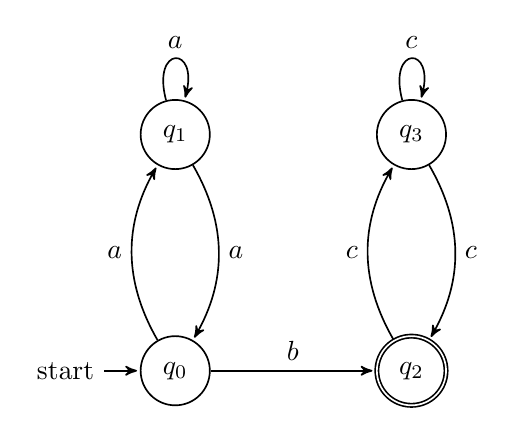
\begin{tikzpicture}[->,>=stealth',shorten >=1pt,auto,node distance=3cm,
        semithick]
      \node[initial,state] (q0) {$q_0$};
      \node[state] (q1) [above of=q0] {$q_1$};
      \node[state,accepting] (q2) [right of=q0] {$q_2$};
      \node[state] (q3) [above of=q2] {$q_3$};
      \path (q0) edge [bend left] node {$a$}(q1)
      edge node {$b$} (q2)
      (q1) edge [loop above] node {$a$} (q1)
      edge [bend left] node {$a$} (q0)
      (q2) edge [bend left] node {$c$} (q3)
      (q3) edge [loop above] node {$c$} (q3)
      edge [bend left] node {$c$} (q2);
    \end{tikzpicture}
  \end{center}\ \\
  \begin{center}
    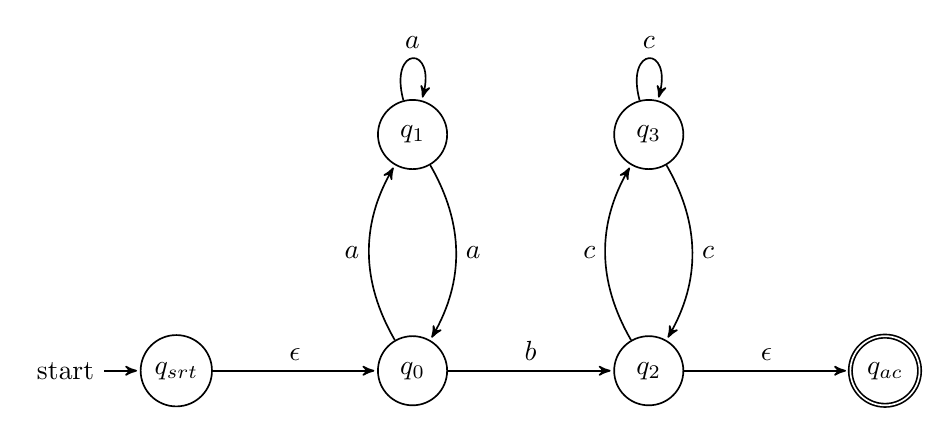
\begin{tikzpicture}[->,>=stealth',shorten >=1pt,auto,node distance=3cm,
        semithick]
      \node[initial,state] (qs1){$q_{srt}$};
      \node[state] (q01) [right of = qs1]{$q_0$};
      \node[state] (q11) [above of=q01] {$q_1$};
      \node[state] (q21) [right of=q01] {$q_2$};
      \node[state] (q31) [above of=q21] {$q_3$};
      \node[state,accepting] (qa1) [right of=q21] {$q_{ac}$};
      \path (qs1) edge node {$\epsilon$} (q01)
      (q01) edge [bend left] node {$a$} (q11)
      edge node {$b$} (q21)
      (q11) edge [loop above] node {$a$} (q11)
      edge [bend left] node {$a$} (q01)
      (q21) edge [bend left] node {$c$} (q31)
      edge node {$\epsilon$} (qa1)
      (q31) edge [loop above] node {$c$} (q31)
      edge [bend left] node {$c$} (q21);
    \end{tikzpicture}
  \end{center} \ \\
  \begin{center}
    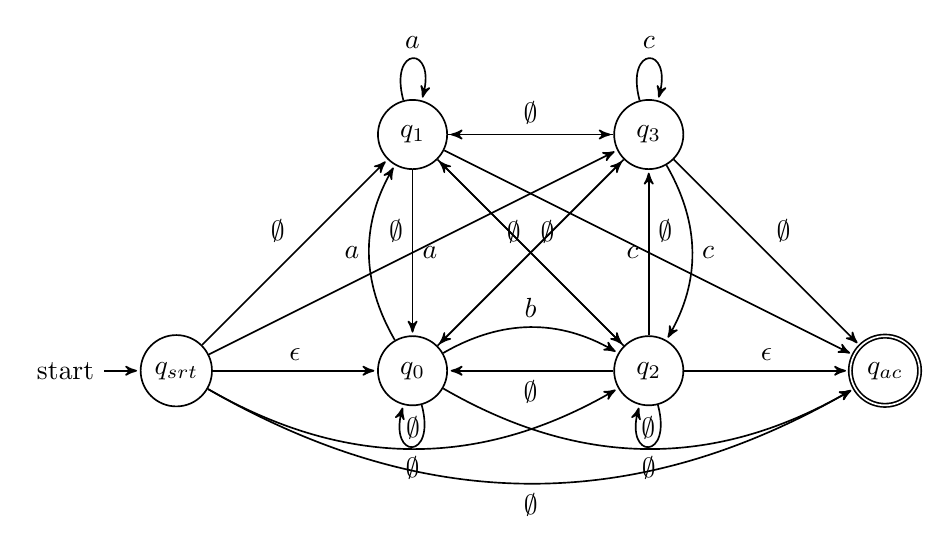
\begin{tikzpicture}[->,>=stealth',shorten >=1pt,auto,node distance=3cm,
        semithick]
      \node[initial,state] (qs1){$q_{srt}$};
      \node[state] (q01) [right of = qs1]{$q_0$};
      \node[state] (q11) [above of=q01] {$q_1$};
      \node[state] (q21) [right of=q01] {$q_2$};
      \node[state] (q31) [above of=q21] {$q_3$};
      \node[state,accepting] (qa1) [right of=q21] {$q_{ac}$};
      \path (qs1) edge node {$\epsilon$} (q01)
      edge node {$\emptyset$} (q11)
      edge node {$\emptyset$} (q31)
      edge [bend right] node {$\emptyset$} (q21)
      edge [bend right] node [below] {$\emptyset$} (qa1)
      (q01) edge [bend left] node {$a$} (q11)
      edge [bend left] node {$b$} (q21)
      edge node {$\emptyset$}(q31)
      edge [loop below] node {$\emptyset$}(q01)
      edge [bend right] node {$\emptyset$}(qa1)
      (q11) edge [loop above] node {$a$} (q11)
      edge node {$a$} (q01)
      edge node {$\emptyset$} (q31)
      edge node {$\emptyset$} (qa1)
      edge node {$\emptyset$} (q21)
      (q21) edge node {$c$} (q31)
      edge node {$\epsilon$} (qa1)
      edge node {}(q11)
      edge node {$\emptyset$}(q01)
      edge [loop below] node {$\emptyset$}(q21)
      (q31) edge [loop above] node {$c$} (q31)
      edge node {} (q11)
      edge node {} (q01)
      edge node {$\emptyset$} (qa1)
      edge [bend left] node {$c$} (q21);
    \end{tikzpicture}
  \end{center}
  \caption{Three-step guide to constructing the GNFA from the DFA}
\end{figure}

Now as that is done, we match triangular figures \footnote{Where node a is connected to c and b, and b is connected to c. We can in such a case remove node b and extend the expresion between a and c with the union of every that earlier was on the path a->b->c.} and remove edges.\\
Look at the edges going between $q0$ and $q1$ where $q0$ is both a and c to reference the above. And since all the other edges are empty transactions, theese do not have to be put into account.
Do the same with $q2$ and $q3$, and get the following atomaton.
\begin{center}
  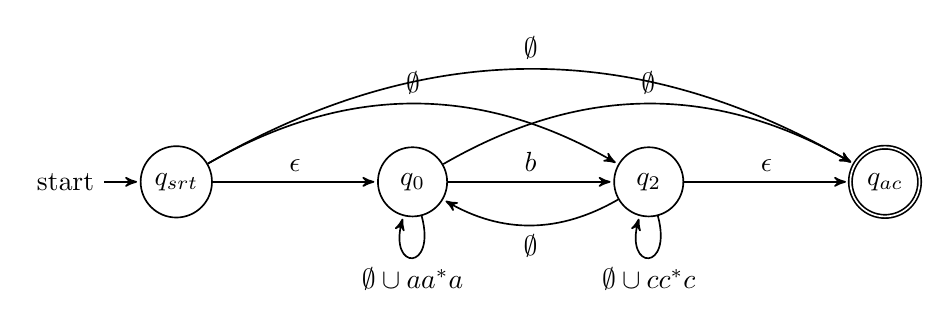
\begin{tikzpicture}[->,>=stealth',shorten >=1pt,auto,node distance=3cm,
      semithick]
    \node[initial,state] (qs1){$q_{srt}$};
    \node[state] (q01) [right of = qs1]{$q_0$};
    \node[state] (q21) [right of=q01] {$q_2$};
    \node[state,accepting] (qa1) [right of=q21] {$q_{ac}$};
    \path (qs1) edge node {$\epsilon$} (q01)
    edge [bend left] node {$\emptyset$} (q21)
    edge [bend left] node {$\emptyset$} (qa1)
    (q01)
    edge node {$b$} (q21)
    edge [loop below] node {$\emptyset \cup aa^*a$}(q01)
    edge [bend left] node {$\emptyset$}(qa1)
    (q21)
    edge node {$\epsilon$} (qa1)
    edge [bend left] node {$\emptyset$}(q01)
    edge [loop below] node {$\emptyset \cup cc^*c$}(q21);
  \end{tikzpicture}
\end{center}

Now removing $q2$ by the same method

\begin{center}
  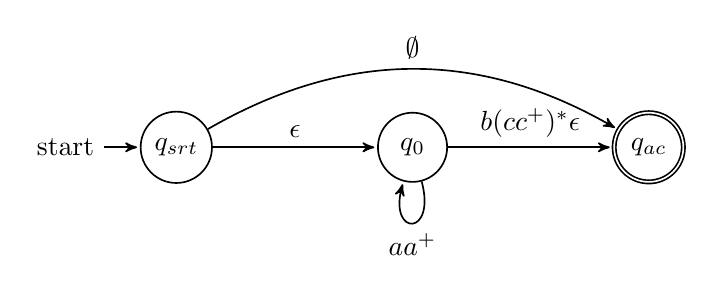
\begin{tikzpicture}[->,>=stealth',shorten >=1pt,auto,node distance=3cm,
      semithick]
    \node[initial,state] (qs1){$q_{srt}$};
    \node[state] (q01) [right of = qs1]{$q_0$};
    \node[state,accepting] (qa1) [right of=q01] {$q_{ac}$};
    \path (qs1) edge node {$\epsilon$} (q01)
    edge [bend left] node {$\emptyset$} (qa1)
    (q01)
    edge [loop below] node {$aa^+$}(q01)
    edge node {$b(cc^+)^*\epsilon$}(qa1);
  \end{tikzpicture}
\end{center}

At last removing $q0$ and getting
\begin{center}
  \begin{tikzpicture}[->,>=stealth',shorten >=1pt,auto,node distance=3cm,
      semithick]
    \node[initial,state] (qs1){$q_{srt}$};
    \node[state,accepting] (qa1) [right of=q01] {$q_{ac}$};
    \path (qs1) edge node {$(aa^+)^*b(cc^+)^*$} (qa1);
  \end{tikzpicture}
\end{center}

And there we have it, $(aa^+)^*b(cc^+)^*$, the regular expressing defining the language that the DFA accepts.

\subsection{Problem 1d}
\begin{align*}
  \{w\mid \text{$w$ contains equally many occurences of the substrings 01 and 10}\}.
\end{align*}

Assume that this means that 010 is accepted expression since both 01 and 10 are substrings of 010.
What this really means is that there is an equal number of changes from 0 to 1 and from 1 to 0. We can easily see that one can not go more than one ahead in change. Since the change $0 \rightarrow 1$ is not possible more than one time before the change $1\rightarrow 0$ has to  be done to performe the $0 \rightarrow 1$ change again. One can also think the automaton accepts all strings that start and end with the same symbol. \\
The DFA will also accept the empty string since the occurance of 01 and 10 both are 0, and thereby equal.
\begin{center}
  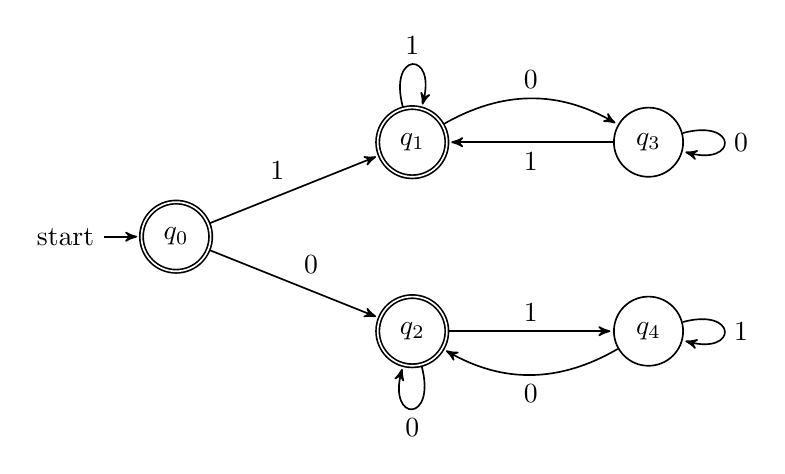
\begin{tikzpicture}[->,>=stealth',shorten >=1pt,auto,node distance=3cm,
      semithick]
    \node[initial, accepting, state] (q0){$q_{0}$};
    \node[state, accepting] (q1) [right of = q0, yshift = 1.2cm]{$q_1$};
    \node[state, accepting] (q2) [right of = q0, yshift = -1.2cm] {$q_2$};
    \node[state] (q3) [right of=q1] {$q_{3}$};
    \node[state] (q4) [right of=q2] {$q_{4}$};
    \path (q0) edge node {$1$} (q1)
    edge node {$0$} (q2)
    (q1)
    edge [bend left] node {$0$} (q3)
    edge [loop above] node {$1$}(q1)
    (q2)
    edge node {$1$} (q4)
    edge [loop below] node {$0$}(q2)
    (q3)
    edge  node {$1$} (q1)
    edge [loop right] node {$0$}(q3)
    (q4)
    edge [bend left] node {$0$} (q2)
    edge [loop right] node {$1$}(q1);
  \end{tikzpicture}
\end{center}


\section{Problem 2: all-NFAs}
Assume that you have an all-NFA G that you want to convert to a DFA $D = (Q_D, \Sigma, \delta_D, q_{1_D}, F_D)$. \\ \ \\
Let $G' = (Q, \Sigma , \delta, q_1, F')$ be an NFA with the same properties as G, except for F, the finish state. The difference between G an G' is that G accepts only those inputs where all the computational branches are at an accept state, whereas G' accepts as long as at least one is.

Since G' is an NFA we know we can convert G' to a DFA $D' = (Q_{D'}, \Sigma, \delta_{D'}, q_{1_{D'}}, F_{D'})$ where D' has the following properties:
\begin{figure}[H]
\begin{align*}
  Q_{D'} &= \mathcal{P}(Q)\\
  \delta_{D'}(R, a) &= \{q\in Q | q \in \delta(r, a) \text{ for some } r \in R \} \qquad R \in Q_{D'} \\
  q_{0_{D'}} &= \{q_0\} \\
  F_{D'} &= \{R \in Q_{D'} | R \text{ contains an accept state }N \}
\end{align*}
\caption{Credit to book}
\end{figure}

To make D' into D, we want to remove all states that have lead to at least one branch dying out, and the connecting transactions to this state.

\begin{enumerate}
\item Let D = D', and we will start removing posibillites from D.
\item For every state $q \in Q_D$ and $p \in Q_D$, given $a \in \Sigma, \, \delta_{D_{q,p}}(q, a) = p$  \\
  then for every $q' \in q$ look at all leagal transitions given $a$. If any of them leads to a termenating branch, make $q$ a sink state  and remove the transition $\delta_{D_{q,p}}(q, a) = p$.
\item Remove any state but the start state that has no incomming transactions.
\item Repeat step 2 and 3 until done.
\item For all states $f \in F$, if there is an $f' \in f$ that is not an accept state, make f non-accepting as well.  
\end{enumerate}






\section{Problem 3: Non-regular languages}
\subsection{Problem 3a}

\begin{center}
  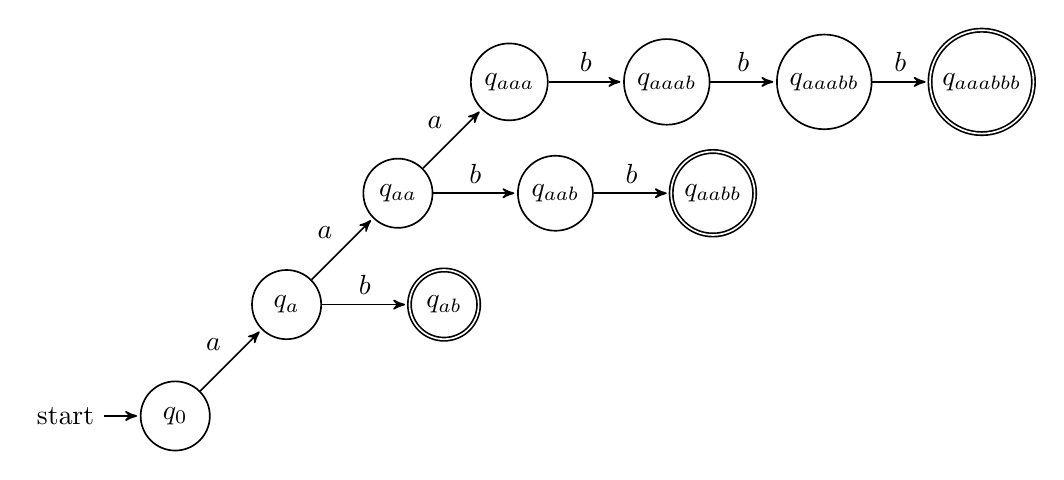
\begin{tikzpicture}[->,>=stealth',shorten >=1pt,auto,node distance=2cm,
      semithick]

    \node[initial,state] (q0) {$q_0$};
    \node[state] (qa) [above right of=q0] {$q_{a}$};
    \node[state,accepting] (qab) [right of=qa] {$q_{ab}$};
    \node[state] (qaa) [above right of=qa] {$q_{aa}$};
    \node[state] (qaaa) [above right of = qaa] {$q_{aaa}$};
    \node[state] (qaaab) [right of = qaaa] {$q_{aaab}$};
    \node[state] (qaaabb) [right of = qaaab] {$q_{aaabb}$};
    \node[state, accepting] (qaaabbb) [right of = qaaabb] {$q_{aaabbb}$};
    \node[state] (qaab) [right of=qaa] {$q_{aab}$};
    \node[state,accepting] (qaabb) [right of=qaab] {$q_{aabb}$};

    \path (q0) edge node {$a$} (qa)
    (qa) edge node {$b$} (qab)
    edge node {$a$} (qaa)
    (qaa) edge node {$b$} (qaab)
    edge node {$a$} (qaaa)
    (qaab) edge node {$b$} (qaabb)
    (qaaa) edge node {$b$} (qaaab)
    (qaaab) edge node {$b$} (qaaabb)
    (qaaabb) edge node {$b$} (qaaabbb);
  \end{tikzpicture}
\end{center}
defines the language $\{ab,aabb, aaabbb\}$.



\subsection{Problem 3b}
I assume that by determenistic infinite automaton, a determenistic pushdown automaton suffice, since the stack in such have an infinite storage amount.
\begin{align*}
  \{a^n b^n\mid n\in\mathbb N\}.
\end{align*}

Let the PDA be described as follows:
\begin{align*}
  Q &= \{q_0, q_1, q_2, q_3 \}\\
  \Sigma &= \{a,b\} \\
  \Upgamma & = \{\$, a\}\\
  q_0 &= q_0 \\
  Z\footnotemark &= \epsilon\\
  F &= \{q_0, q_3\}
\end{align*}
\footnotetext{Initial state in the stack}
Let $\delta : (Q \times \Sigma \times \Upgamma) \rightarrow (Q \times \Upgamma)$ be defined as the transaction function visible in the representation below.

\begin{center}
  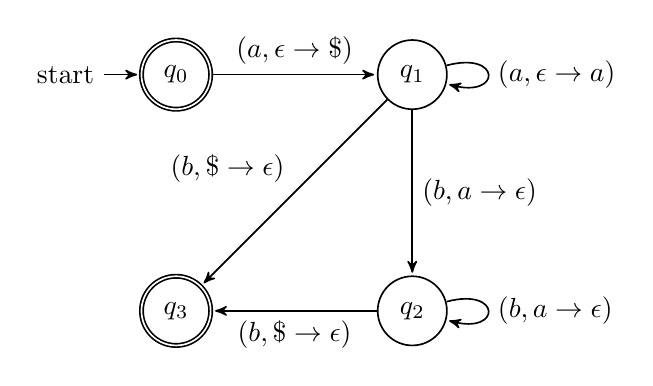
\begin{tikzpicture}[->,>=stealth',shorten >=1pt,auto,node distance=3cm,
      semithick]

    \node[initial,state, accepting] (q0) {$q_0$};
    \node[state] (q1) [right of=q0] {$q_{1}$};
    \node[state] (q2) [below of=q1] {$q_{2}$};
    \node[state, accepting] (q3) [left of=q2] {$q_{3}$};

    \path (q0) edge node {$(a, \epsilon \rightarrow \$) $} (q1)
    (q1) edge [loop right] node {$(a, \epsilon \rightarrow a)$} (q1)
    edge node {$(b, a \rightarrow \epsilon)$} (q2)
    edge node [above left] {$(b, \$ \rightarrow \epsilon)$} (q3)
    (q2) edge [loop right] node {$(b, a \rightarrow \epsilon)$} (q2)
    edge node {$(b, \$ \rightarrow \epsilon)$} (q3);
  \end{tikzpicture}
\end{center}

One might at first glance think this automaton is non-determenistic because of the multiple transactions for $b$ both at $q_1$ and $q_2$.
But with a closer look we see that pop-requests to the stack are all uniqe given an inputsymbol, and no ``choice'' is possible anywhere in the automaton, i.e. the PDA is also an DPDA.
\\ \ \\
And there you have it; an determenistic infinite automaton that accepts the language $\{a^nb^n| n \in \mathbb{N}\}$ \footnote{Strictly speaking it is not a perfect DPDA since not all possible inputs at any state are acounted for, forr exsample $a$ in $q_2$. All transactions that are not drawn all go to a sick state. But due to readability I have chosen to leave this out of the oblig.}



\subsection{Problem 3c}
The pumpinglemma states that any string longer than the pumping length can be pumped. I.e. this means that the automaton contains at least one loop.

Given the language $\{a^nb^n | n \in \mathbb{N}\}$ prove that at least one string in this language cannot be pumped.

\begin{proof}
  Asssume $\{a^nb^n | n \in \mathbb{N}\}$ is a regular language. Let the pumping length be of length $p$. Lets look at the string; $a^pb^p$, which has a length $2p$. Since $2p> p$, this string should, by the pumpinglemma, be pumpable.
  We will, however, show that it cannot be pumped, and thereby proove that the language is irragular.
  Since the string $a^pb^p$ can be pumped, it can be devided into 3 parts $xy^iz$ where $y$ is the part that gets pumped. We also know that $|y| > 0$ and $|xy| \leq p$. With this in mind we can look at all possible ways $a^pb^p$ can be divided.

  \textbf{Case 1: y = some number of a's.}\\
  Since y can be pumped, the number of a's increase, but the number of b's stay the same. The number of a's is greater than the number of b's after pumping. Case 1 is not pumpable. \\
  \textbf{Case 2: y = some number of a's and b's.}\\
  Since $|xy| \leq p$ and $|a^p| = p$ then this is not a valid selection of y. \\
  \textbf{Case 3: y = some number of b's.}\\
  This is only a more extreme version of Case 2 and is no leagal selection of y.


  Since we have found one occurance of a string in the language $\{a^nb^n | n \in \mathbb{N}\}$ with length longer than the pumping length, but cannot be pumped, we have prooven that the language is non-regular.

\end{proof}






\subsection{Problem 3d}
Show that $\{a^nb^n | n \in \mathbb{N}\}$ is context-free.
\begin{proof}
A language is context free iff there exists a PDA that accepts the same language. And since we in Problem 3b found such a PDA (DPDA) we know that the language $\{a^nb^n | n \in \mathbb{N}\}$ is context-free.
\end{proof}
\end{document}
